\documentclass{article}

\usepackage[utf8]{inputenc}
\usepackage[T1]{fontenc}
\usepackage{microtype}

\usepackage{newspaper}

\date{17-nov-1930}
%\date{\today}
\currentvolume{1}
\currentissue{1}

%% [LianTze] The newspaper package also provides 
%% these commands to set various metadata:

%% The banner headline on the first page
%%   (The colon after s: is to get a more
%%   modern majuscule s in this font instead of 
%%   the medieval tall s. For anyone interested 
%%   in the history: 
%%  http://medievalwriting.50megs.com/scripts/letters/historys.htm)
\SetPaperName{Monatshefte}

%% The name used in the running header after
%% the first page
%\SetHeaderName{Monatshefte für Mathematik}
\SetHeaderName{Monatshefte}

%% and also...
\SetPaperLocation{Königsberg GER}
\SetPaperSlogan{``Monatshefte für Mathematik: O seu canal de divulgação matemática.''}
\SetPaperPrice{Três Reais}


% [LianTze] times (the package not the font) is rather outdated now; use newtx (see later)
% \usepackage{times}
\usepackage{graphicx}
\usepackage{multicol}

\usepackage{picinpar}
%uasage of picinpar:
%\begin{window}[1,l,\includegraphics{},caption]xxxxx\end{window}


%% [LianTze] Contains some modifications
\usepackage{newspaper-mod}
%%... so now you can redefine the headline and byline style if you want to.
%% These can be issued just before any
%% byline or headline in the paper, to
%% individually style each article
%%
% \renewcommand{\headlinestyle}{\itshape\Large\lsstyle}
% \renewcommand{\bylinestyle}{\bfseries\Large\raggedright}


%%%%%%%%%  Front matter   %%%%%%%%%%

\usepackage{lipsum}

\begin{document}
\maketitle

\begin{multicols}{3}

    \byline{Primeiro teorema da incompletude}{Peter Norak}

    Teorema 1: \emph{"Qualquer teoria axiomática recursivamente enumerável e capaz de expressar algumas verdades básicas de aritmética não pode ser, ao mesmo tempo, completa e consistente. Ou seja, em uma teoria consistente, sempre há proposições que não podem ser demonstradas nem verdadeiras, nem falsas."}. Teorema 2: \emph{"Uma teoria, recursivamente enumerável e capaz de expressar verdades básicas da aritmética e alguns enunciados da teoria da prova, pode provar sua própria consistência se, e somente se, for inconsistente."}
    \begin{window}[2,r,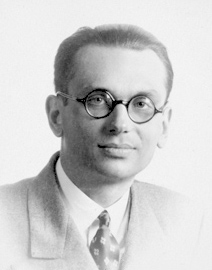
\includegraphics[width=1.0in]{images/kurt.jpg},\centerline{David Hilbert}]  
    A surpreendente prova de Gödel mostrou que a suposição de \emph{Hilbert}, de que toda a matemática pode ser demonstrada a partir de um conjunto finito de axiomas estava errada.
    \end{window}
    %First Incompleteness Theorem: "Any consistent formal system F within which a certain amount of elementary arithmetic can be carried out is incomplete; i.e., there are statements of the language of F which can neither be proved nor disproved in F." (Raatikainen 2015)

%\begin{window}[2,r,\includegraphics[width=1.0in]{atom.jpg},\centerline{The Atom}] The \verb+multicol+ package allows using multiple columns without starting a new page.  Using floats is not possible in a columns environment, however with the \verb+picinpar+ package, I can set a picture inside a block of text---just like you one you see here.  Isn't \LaTeX{} cool?
%And now we're just filling more space, and yet more space.  
%\end{window}
    \closearticle

    \byline{O Paradoxo de Russel}{Richard Stallman}
    \begin{window}[2,r,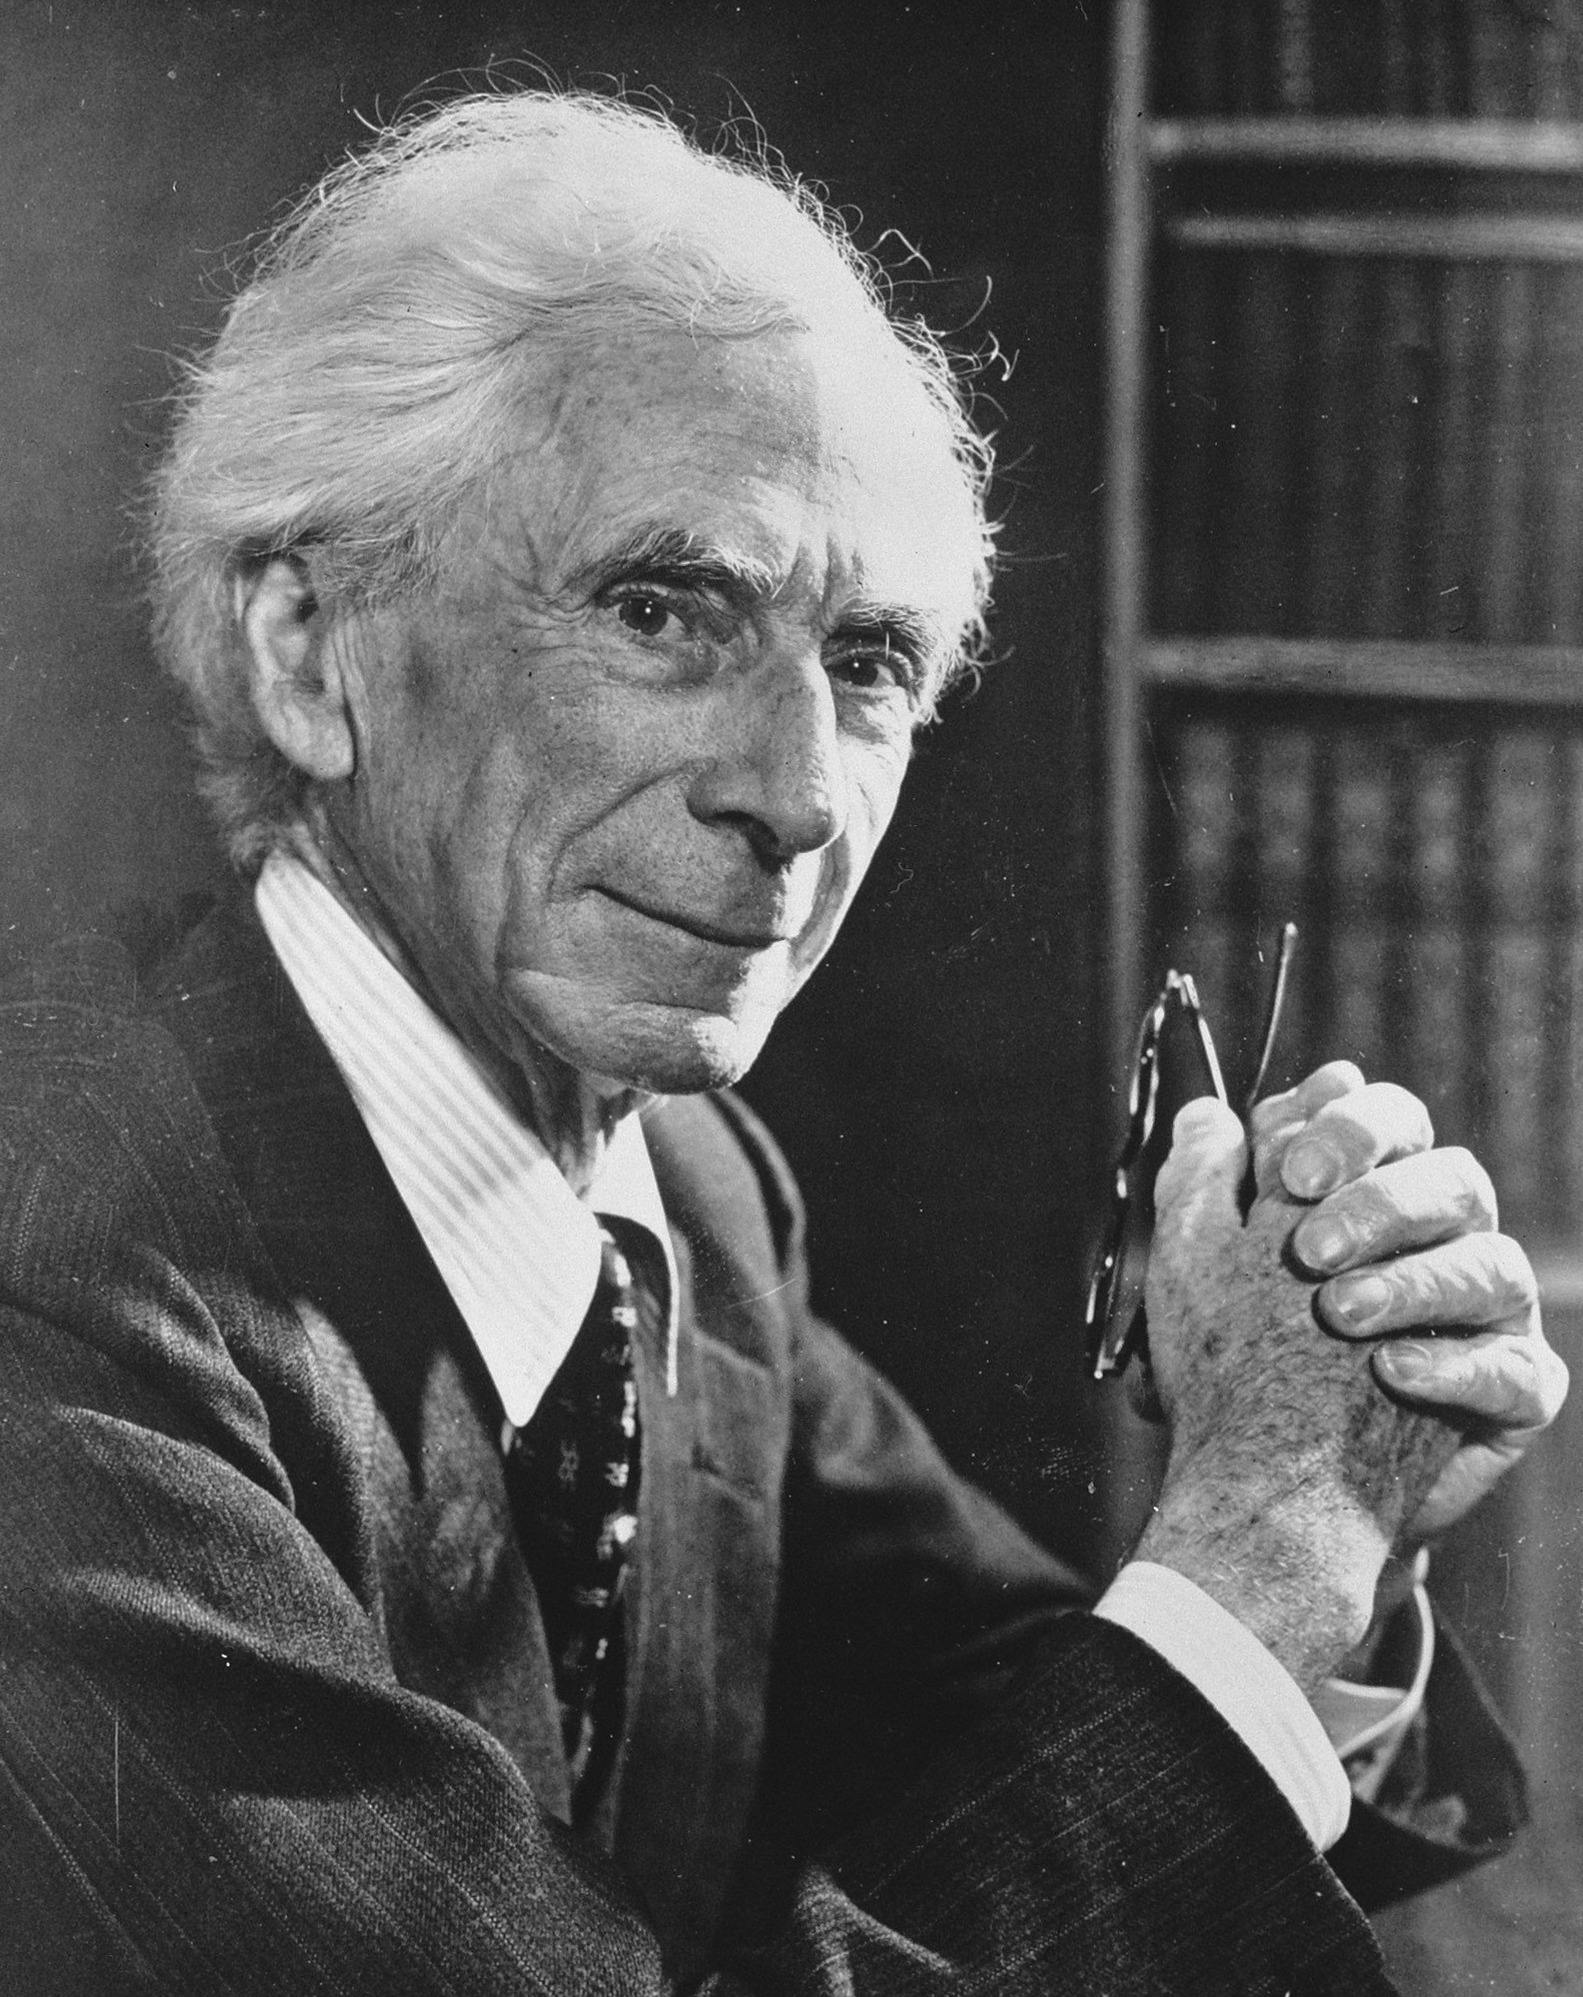
\includegraphics[width=1.0in]{images/russel.jpg},\centerline{Bertrand Russel}]  
    O conhecido paradoxo é posto da seguinte maneira: \emph{Consideremos o conjunto de todos os conjuntos que não tem a si próprio como elemento, ou seja, $D = \{X | X \not\in X\}$}. O paradoxo pode ser obtido quando questionado: $D$ percente a $D$? Se supormos que $D$ pertence a $D$ e observarmos a regra de definição do conjunto, temos $D \not\in D$. Por outro lado, se inicialmente supormos que $D$ não pertence a $D$, ele satisfaz a regra de definição do conjunto e consequentemente $D \in D$, o que contradiz nossa suposição. O paradoxo do barbeiro, é uma maneira ilustrativa daquele paradoxo. Suponhamos que em uma cidade exista \emph{apenas um} barbeiro. Nesta cidade cada homem mantém-se bem barbeado e para isso utiliza-se de exclusivamente um, de dois métodos: $1º)$ Ele vai ao barbeiro. $2º)$ Ele corta sua própria barba. Nesse caso, quem barbeia o barbeiro?
    \end{window}
    \closearticle

    \headline{Programa de Hilbert}{Aische Schmidt}
    \begin{window}[2,r,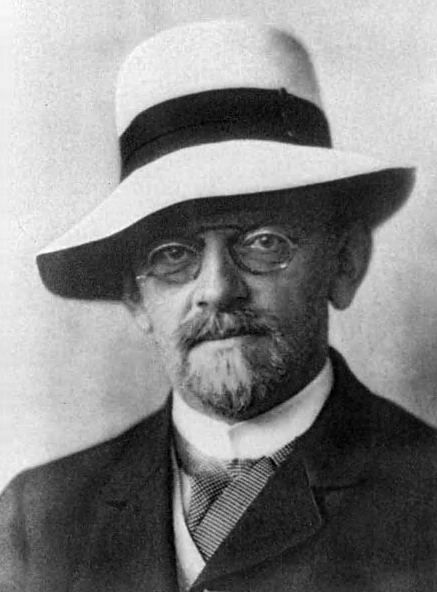
\includegraphics[width=1.0in]{images/hilbert.jpg},\centerline{David Hilbert}] The \verb+multicol+ package allows using multiple columns without starting a new page.  Using floats is not possible in a columns environment, however with the \verb+picinpar+ package, I can set a picture inside a block of text---just like you one you see here.  Isn't \LaTeX{} cool?
And now we're just filling more space, and yet more space.  
    \end{window}
    \closearticle
\end{multicols}
%\newpage
%\begin{multicols}{3}
%    \byline{Programa de Hilbert}{Alfaiate}
%\en:w

\end{document}
